\documentclass{article}
\usepackage{fullpage}
\usepackage{parskip}
\usepackage{hyperref}
\usepackage{listings}
\usepackage{graphicx}
\usepackage{amssymb}
\usepackage{mdwlist}
\usepackage{textcomp}
\usepackage[usenames,dvipsnames]{color}
\hypersetup{
    colorlinks,
    citecolor=Red,
    linkcolor=Red,
    urlcolor=Red}
\begin{document}

\title{Assignment 1: Hello World and Then Some}
\author{CS148 Fall 2015-2016}
\date{}
\maketitle

\section*{Introduction}

\begin{figure}[h!]
    \centering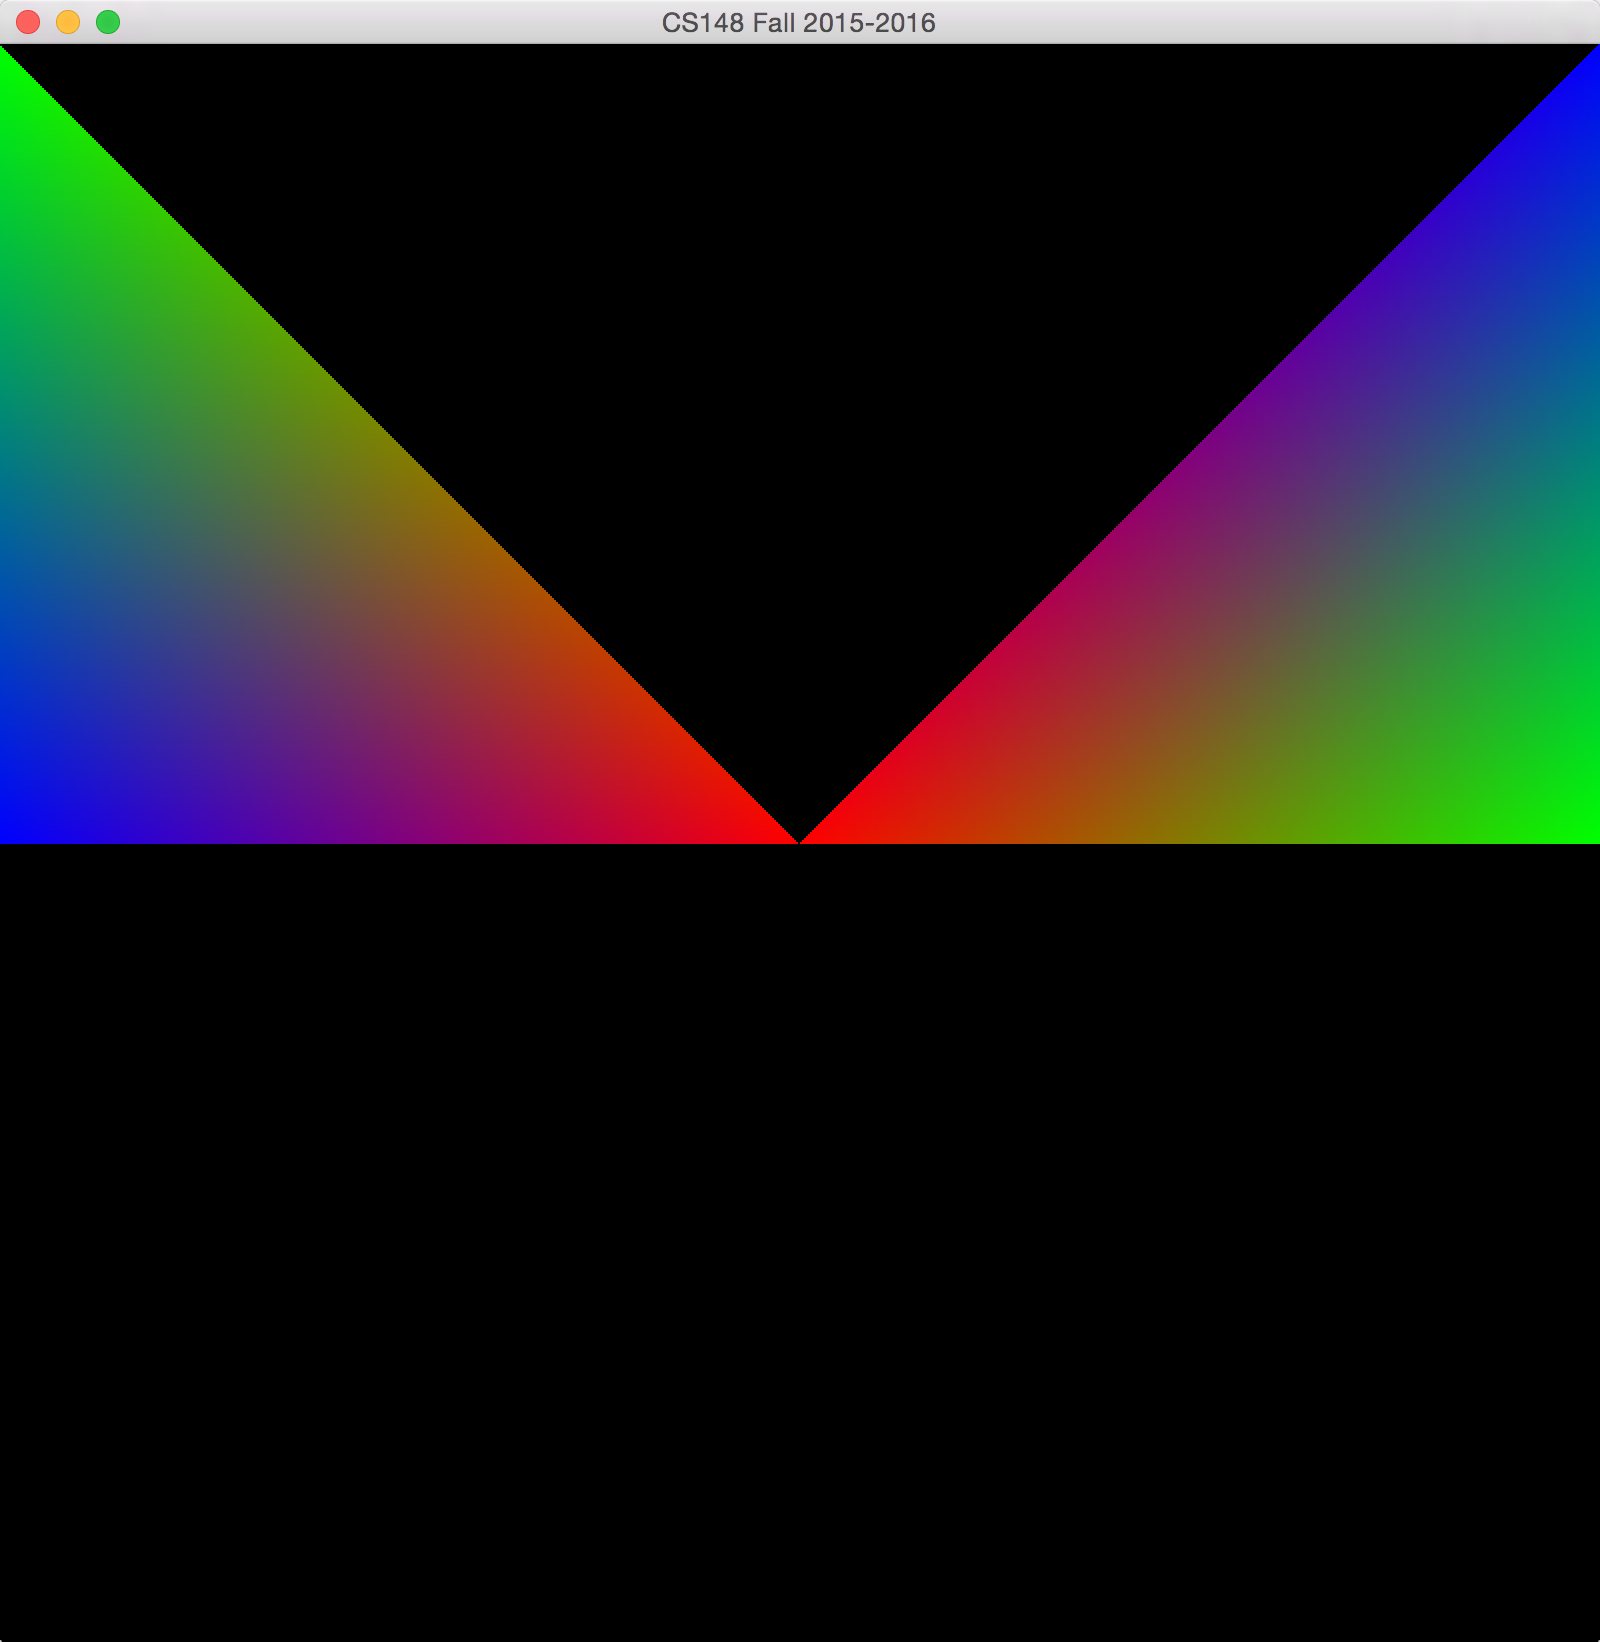
\includegraphics[width=0.5\linewidth]{assign1.png}
    \caption{Just the usual OpenGL "Hello World" triangles}
\end{figure}

If you have not already, make sure you have downloaded the assignemt framework and have gotten it to compile! See the setup guide if you have not done so already. This assignment is meant to give you a gentle introduction to OpenGL 4 and the assignment framework (as well as give you time to work out all the kinks with configuring and compiling for your system!). After completing this assignment, you should:

\begin{enumerate*}
    \item Understand what SDL does with regards to using OpenGL.
    \item Be familiar with how SDL processes mouse/keyboard events and how to send them to your program.
    \item Know how OpenGL 4 takes a bunch of vertices and displays colors on your screen as well as the role of vertex and fragment shaders in this process.
    \item Know your way around GLSL syntax and be comfortable with passing vertex attributes and uniforms to the shader.
\end{enumerate*}

The assignment framework is fairly large so we encourage you to start EARLY and ask questions in office hours and/or Piazza if you get stuck and need help.

\subsection*{Useful Resources}

\begin{enumerate*}
    \item OpenGL Programming Guide Chapters 1-3 (the book is not required, but recommended!)
    \item OpenGL 4 Documentation: \href{https://www.opengl.org/sdk/docs/man4/}{here}. Note that these pages are for OpenGL 4.5 but most should be equivalent (unless otherwise noted on the function's page).
    \item SDL 2 Documentation: \href{https://wiki.libsdl.org/CategoryAPI}{here}.
    \item GLSL Tutorial: \href{http://www.lighthouse3d.com/tutorials/glsl-tutorial/}{here}.
    \item GLM: \href{http://glm.g-truc.net/0.9.7/glm-0.9.7.pdf}{Manual} and \href{http://glm.g-truc.net/0.9.7/api/index.html}{Documentation}.
    \item C++ Reference: \href{http://en.cppreference.com/w/}{here}
    \item Assignment Framework Documentation: This can be found in "source/doxygen"
\end{enumerate*}

\section*{Assignment}

Before starting to write your program, you will need to decide what you want to draw using OpenGL. Here are some ideas (and links to examples and definitions in red) to get you started.
\begin{itemize*}
\item \href{http://mathworld.wolfram.com/Spirograph.html}{Spirographs} or similar functions
\item Fractals, drawn to a certain level, see e.g. the \href{http://en.wikipedia.org/wiki/Koch_snowflake}{Koch Snowflake}
\item Simple \href{http://en.wikipedia.org/wiki/Space-filling_curve}{space filling curves}
\item Simple \href{http://en.wikipedia.org/wiki/L-system}{L-systems}, e.g. use them to create simple trees (lines for branches, triangles for leaves)
\item \href{http://en.wikipedia.org/wiki/Conway's_Game_of_Life}{Conway's game of life}
\item A simple arcade game - Pong, Pacman, Snake...
\item \href{http://www.jwz.org/xscreensaver/screenshots/}{XScreenSaver} has many good examples
\item If you are feeling adventurous, try something with \href{http://9elements.com/io/projects/html5/canvas/}{animation and/or particle effects}, add \href{http://hakim.se/experiments/html5/magnetic/02/}{physics}, and/or try adding some \href{http://hakim.se/experiments/html5/particles/02/}{user input}. These linked examples were done in JavaScript, but you could easily make something similar with OpenGL and some creativity!
\end{itemize*}

\subsection*{Assignment 1 Code Explanation}

Look in the Assignment1 class documentation in the assignment framework documentation found at "source/doxygen".

\subsection*{Shader Loading}

Shaders are stored in the "shaders" folder. When the program is compiled, a script is run to copy this folder into the right location. As a result, to load a shader, you only have to specify the shader path relative to the shaders folder. For example, for the vertex shader located at "shaders/basicColor/basicColor.vert", Assignment1.cpp only tells the framework to load the shader from "basicColor/basicColor.vert". If you make new shaders, make sure they are in the shaders folder!

\subsection*{Pointers to Get You Started}
\begin{itemize*}
\item Without transformations, the coordinates of your scene will be equivalent to the "normalized device coordinates" which has the top left corner coordinate as $(-1, 1)$ and the bottom right corner coordinate as $(1, -1)$.
\item Look in "source/common/MediaLayer.h/cpp" to see how OpenGL and SDL are setup, in particular the InitializeOpenGL and InitializeSDL functions.
\item Look in "source/common/MediaLayer.h/cpp" to see how SDL handles events (i.e. keyboard) in the 'Tick' function. You will need to modify this function if you want to use the mouse in your program! The SDL\_Event \href{https://wiki.libsdl.org/SDL_Event}{documentation} may be helpful.
\item To see how the framework takes in your vertices and whatever else and sets it up to display on the screen look in "source/common/Rendering/RenderingObject.h/cpp". The "UpdateVertexXYZ" functions takes in the raw data and passes it to OpenGL. The BeginRender(), Render(), and EndRender() functions performs setup/drawing/teardown during the rendering loop. Questions about a specific OpenGL function? Look it up in the documentation first (linked in "Useful Resources" above). Still confused? Ask a CA!
\item "std::unique\_ptr \textlangle T\textrangle" and "std::shared\_ptr \textlangle T\textrangle" are special types of pointers introduced in C++11. Using "std::shared\_ptr\textlangle T\textrangle" gets you reference counting and thus lets you (for the most part) not worry about deallocating memory. Using "std::unique\_ptr\textlangle T\textrangle" is similar except that you can not make a copy of a unique pointer! The pointer has to be unique! Thus, if you want to "transfer ownership" somewhere else, you will have to use std::move (you will see alot of this in the code) which will invoke the \href{http://en.cppreference.com/w/cpp/language/move_constructor}{move constructor} (should you pass the unique pointer to a function or otherwise assign it). After doing so, the original unique pointer will no longer be valid!
\item If you want to modify the shaders, you will want to do so in the "source/shaders/basicColor" folder. 
\end{itemize*}

\subsection*{Tips and Tricks}
\begin{itemize*}
\item While developing it will be useful to compile your program in "Debug" mode. This will enable the assertions in the code to help you debug. Additionally, it will enable the OGL\_CALL macro to do an OpenGL error check which can provide useful information if nothing is showing up on your screen!
\item Want circular points instead of square ones? Look into \href{https://www.opengl.org/sdk/docs/man/html/gl_PointCoord.xhtml}{gl\_PointCoord}! The "Point Sprites" section of Chapter 6 of the OpenGL Programming Guide (Red Book) is useful too!
\end{itemize*}

\section*{Questions}
\begin{enumerate*}
\item Explain how a "Vertex Array Object" and a "Vertex Buffer Object" are related.
\item Which OpenGL calls relate to the generation and usage of a "Vertex Array Object" and which relate to the generation and usage of a "Vertex Buffer Object".
\item How does OpenGL know whether you want to draw a triangle, line, point or other some other primitive?
\end{enumerate*}

\section*{Feedback (Optional)}
\begin{enumerate*}
\item On a scale of 1-10 [10 being very clear]: How clear were the instructions to configure and compile the assignment framework?
\item On a scale of 1-10 [10 being the most work]: How much work was this assignment (including configuring and compiling the project)?
\item On a scale of 1-10 [10 being very easy to use]: How understandable/easy to use is the assignment framework?
\item How much experience with C++ and OpenGL did you have before taking the course?
\end{enumerate*}

\section*{Grading}
This assignment will be graded on the following requirements
\begin{itemize*}
\item The program draws using at least two of the OpenGL primitives in at least two different colors.
\item The program incorporates some form of user interaction.
\item The student is able to adequetely answer questions asked by the CAs.
\item The student's vertex or fragment shader uses one (or more) uniforms. (optional)
\end{itemize*}
according to the following rubric.
\begin{itemize*}
\item $+$ -- Exceeds the requirements via one or more artistic/technical contributions
\item $\checkmark$ -- Meets all of the requirements
\item $-$ -- Does not meet the requirements but still produces a drawing.
\item $0$ -- The submitted solution does not produce a drawing.
\end{itemize*}

\end{document}

